
As outlined in section \ref{chap_mh_sampler}, the Metropolis Hastings Algorithm can be defined by its posterior probability and $Q(\Theta, \tilde{\Theta})$. The former can be computed recursively as shown in section \ref{chap_math_approach}; so $Q$ remains to be defined.

\textit{Symmetric Proposals}, i.e. proposals where $Q(\Theta, \tilde{\Theta}) = Q(\tilde{\Theta}, \Theta)$, are commonly employed. In absence of prior information indicating otherwise, this choice is natural as it does not arbitrarily favour some parameters over others. A common choice for a symmetric proposal is the normal distribution $\mathcal{N}(0, \sigma^2)$ for some $\sigma > 0$. 


\subsubsection*{Autocorrelation}
The choice of $\sigma$ directly influences the auto correlation the chain's samples will exhibit and hence the effective sample size. In particular, small values of $\sigma$ lead to proposals which are always very close to the current sample, incurring a high auto correlation. On the other hand, if $\sigma$ is too great, then the newly proposed value is likely to be extreme and hence unlikely. This makes the new sample very likely to be rejected. Rejection leads to strings of identical values, which are of course perfectly auto correlated.

Figures \ref{fig:sticky_chain} and \ref{fig:unsticky_chain} show two chains sampled with different choices of $\sigma$ for the same data and proposal distribution. They clearly illustrate how a $\sigma$ chosen too big can lead to poor behaviour of the resulting chain. 


\subsubsection*{Exploration of Search Space}
Small $\sigma$ lead to local suggestions; hence, multi-modal distributions are unlikely to be explored as the chain gets ''stuck'' in local maxima. A commonly used technique known as ''Simulated Annealing'' circumvents this phenomenon by decreasing $\sigma$ in the course of time. In the beginning, chains are then able to explore the search space, whereas later on with a small $\sigma$, they are also likely to zero in on the sought value. 

Please note that in Bayesian Inference, we are interesting in sampling a \textit{distribution} instead of a \textit{point estimate}. Hence, $\sigma$ cannot not be chosen arbitrarily small. 

\begin{figure}
	\begin{subfigure}[b]{0.9\textwidth}
		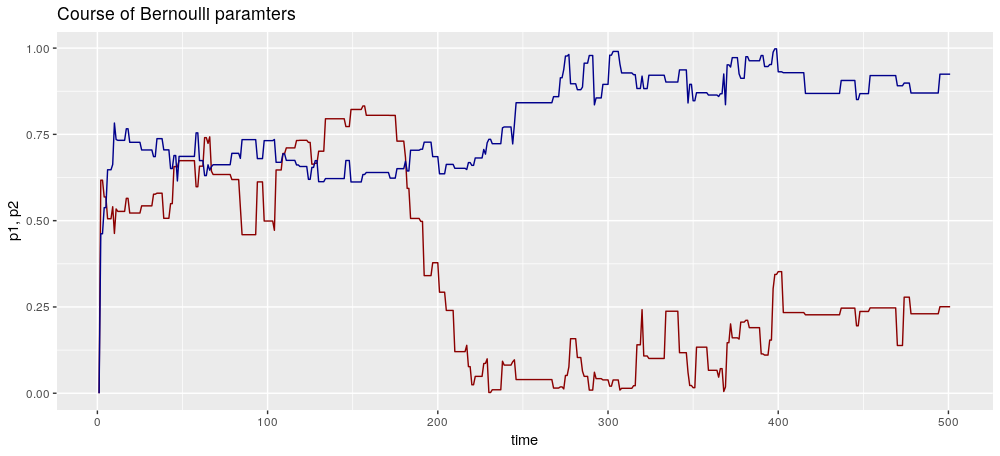
\includegraphics[width=\linewidth]{./img/sticky_chain.png}
		\caption{}
		\label{fig:sticky_chain}
	\end{subfigure}\\
	\begin{subfigure}[b]{0.9\textwidth}
		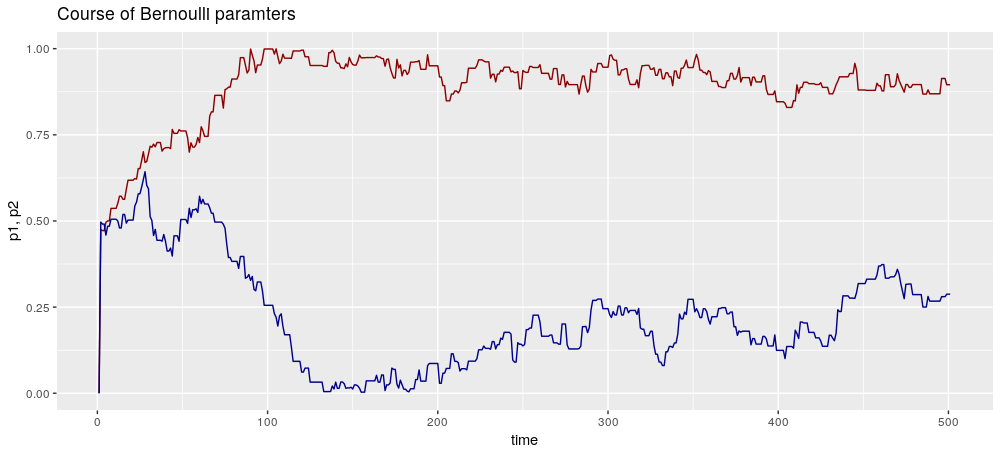
\includegraphics[width=\linewidth]{./img/unsticky_chain.png}
		\caption{}
		\label{fig:unsticky_chain}
	\end{subfigure}
	\caption{In figure \ref{fig:sticky_chain}, the path of the Bernoulli paramters of a Metropolis-Hastings chain with proposals $\mathcal{N}(0, 0.08^2)$ is shown; \ref{fig:unsticky_chain} uses proposals from $\mathcal{N}(0, 0.03^2)$. We can clearly see that the chain in \ref{fig:sticky_chain} is very ''stick'', i.e. often the chain rests with the current sample. On the other hand, the steps its Metropolis-Hastings sampler takes are usually greater than those of the not so sticky chain \ref{fig:unsticky_chain}. } 
\end{figure}


For these reasons, it is important to choose $\sigma$ wisely. Indeed, Johansen \cite{mcnotes} suggests to tweak $\sigma$ such as to obtain an acceptance rate of $0.44$ in the 1-dimensional case and $0.28$ in the multi-dimensional case. Often, those optimisations are performed manually by trial \& error; however, \cite{christen2010} suggests an algorithm adapting $\sigma$ automatically which appears to work well for many practical examples. 


\subsubsection{Modification of acceptance criterion}
As our algorithms work in log space, we modify the acceptance criterion as follows:
\codeBox{Metropolis-Hastings Acceptance Criterion in Log Space}{
	\begin{enumerate}
		\item Let 
		\begin{align}
		\tilde{\alpha} := min \Bigg\{ 0,  log\left( \tip{\tp} \, Q(\tp, \Theta) \right) - log\left( \tip{\Theta} \, Q(\Theta, \tp) \right) 			
		\Bigg\}
		\label{alphaSamplingStep}
		\end{align}
		\item Draw $u \sim U[0, 1]$
		\item If $log(u) \leq \tilde{\alpha}$, accept $\tp$ (i.e. set $\Theta_{t+1} = \tp$), otherwise reject it (i.e. $\Theta_{t+1} = \Theta_t$). 
	\end{enumerate} 
}

\subsection{Constrained Parameters}
For our purposes, $\Theta$ contains $\Gamma, \delta$ and a parameterisation of the states' distributions. Those are typically Bernoulli or Poisson distributions. 

All of those parameters are constrained:
\begin{itemize}
	\item $0 \leq \delta_i \leq 1$ with $\sum \delta_i = 1$ \\
	\item $0 \leq \Gamma_{j, i} \leq 1$ with $ \sum\limits_{i=1}^m \Gamma_{j, i} = 1$ \\
		for all $ 1 \leq j \leq m$
	\item $ 0 \leq p \leq 1$ for Bernoulli distributions or $\lambda \geq 0$ for Poisson distributions
\end{itemize}

When choosing a new proposal $\tilde{\Theta}$ from the current sample $\Theta$, with a step sampled from a normal distribution, it is not immediately clear how to ensure that the new proposal satisfies the constraints. 

The easiest option is to simply reject all samples which are not valid. While incurring a high rejection rate\footnote{Which can be prohibitively high for high-dimensional problems}, this methodology becomes unfeasible if we consider constraints as in (1) above. 


\subsubsection*{Natural and Working Parameters}
A common approach to deal with this is to apply transformations such as the $log$-transformation. For instance, if a parameter is constrained to $[0,1]$, we could work in a transformed space instead. 
For instance, if our algorithm was to suggest values in $(-\infty, \infty)$ (so-called \textit{working parameters}), we could apply the log-transformation to map those values into $[0,1]$ (so-called \textit{natural parameters}); this would ensure that all new proposals are valid from a model point of view. 

However, the steps are usually normally distributed in the space of the natural parameters and it is unclear what the distribution of a random variable $X$ would be s.t. $exp(X) \sim \mathcal{N}(0, \sigma)$. 




\subsubsection*{''Bumping'' of Parameters}
When naiively using a symmetric distribution to obtain a new proposal for a parameter from the current one, we may come up with an invalid proposal. For instance, if the paramter in question is constrained to $[0,1]$, choosing a $\mathcal{N}(0, \sigma)$ step to alter the current sample may yield a proposal outside of these bounds.
 
There are two approaches to this problem: Either, one alters the new proposal such that it corresponds to the constraints, or one uses a sampling method respecting the constraints in a natural way. 
''Bumping'' is a simple methodology for the former. 

Let $p \in [0,1]$ be a parameter and $s: [0,1] \rightarrow \R$ be a function mapping $p$ to a new proposal. Then we draw new samples as follows:
\codeBox{Bumping of parameters}{
	\begin{algorithmic}
			\State $\tilde{p} \gets s(p)$
			\If {$\tilde{p} \in [0, 1]$}
				\State $p \gets \tilde{p}$
			\ElsIf{$min\{ abs(p - 0), abs(1-p) \} < 1$}
				\If {$\tilde{p} < 0$ }
					\State $p \gets - \tilde{p}$
				\Else
					\State $p \gets 1 - (\tilde{p} - 1)$
				\EndIf
			\Else
				\State reject new proposal
			\EndIf
	\end{algorithmic}
}

\begin{figure}
	\centering
	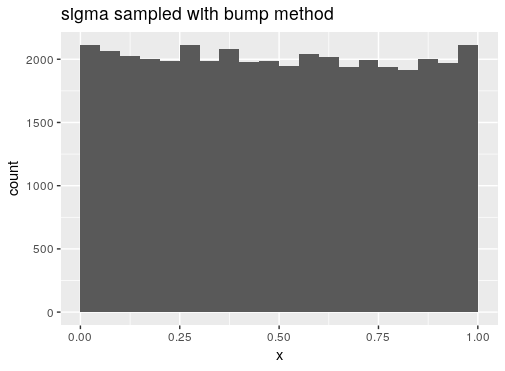
\includegraphics[height = 0.3\textheight]{img/bumpItBaby.png}
	\caption{Sampling of $p \in [0,1]$ with bumping method and $\sigma= 0.1$ for $200$ chains with each $200$ samples. }
	\label{fig:bumpingIsUniform}
\end{figure}

Figure \ref{fig:bumpingIsUniform} shows that sampling with the bumping method does indeed uniformly cover the interval $[0,1]$\footnote{Note that as the sample size increases, the distribution continues to converge towards the uniform distribution. This has been confirmed generating several histograms and verifying that the overall shape attained is consistently almost constant.}
As we shall see, this is not true for many other methods. 

We note the following:
\begin{enumerate}
	\item the interval can easily be generalised
	\item the proposal is symmetric
	\item if the proposed new sample is farther than $1$ away from both $0$ and $1$, the new sample is rejected. The variance of the proposal distribution should be chosen small s.t. this case becomes unlikely.
\end{enumerate}



\subsubsection{Drawing from a constrained distribution}
% source: https://stats.stackexchange.com/questions/142999/simulate-from-a-truncated-mixture-normal-distribution/143011#143011
We would prefer to directly draw a parameter from a distribution which respects the constraints the parameter is subject to over rejecting or bumping a parameter after it has been drawn. 

One way to do so is to use a \textit{truncated normal distribution}.
Let us denote the normal distribution, truncated to the interval $[a, b]$ with $X \sim \mathcal{N}_a^b(\mu, \sigma^2)$. 

\begin{lemma}
	The cdf of $X$ is \\
	\begin{align*}
	F(x) = \begin{cases}
		0	& x \leq  a \\
		\frac{
			\Phi\left( \frac{x - \mu}{\sigma} \right)
			- \Phi\left(\frac{a - \mu}{\sigma}\right)
		}{
		\Phi\left(\frac{b - \mu}{\sigma}\right)
		- \Phi\left(\frac{a - \mu}{\sigma}\right)
		}
	    & \, \text{otherwise}
		\end{cases}
	\end{align*}
	where $\Phi$ is the cdf of a standard normal random variable.
	\label{lem:cdf}
\end{lemma}

\begin{proof}
	Let $\tilde{X} \sim \mathcal{N}(\mu, \sigma^2)$. \\
	Then we have 
	\begin{align*}
		F_{ \tx \, | \, \tx \in [a, b]}(x) &= \frac{\uP{\tx < x \cap \tx \, \in \, [a, b]} }{\uP{\tx \, \in \, [a, b]}} \\
		&= \frac{\uP{\nt{\tx} < \nt{x} \cap \nt{\tx} \, \in \, \left[\nt{a}, \nt{b} \right]} }{\uP{\nt{\tx} \, \in \, [\nt{a}, \nt{b}]}} \\
		&\overset{x \, \geq \, a}{=} \frac{\nd{x} - \nd{a}}{\nd{b} - \nd{a}}
	\end{align*}
\end{proof}

\begin{theorem}[The Inversion Method]
Let $X \sim F$ where $F$ is some cdf and let $F^{-1}$ be the inverse\footnote{or if the inverse does not exist, the pseudo-inverse} of $F$. 
Then
\[
F_X^{-1}(U[0, 1]) \sim X
\]
\end{theorem}

Lemma \ref{lem:cdf} provides us with the cdf of a truncated normal distribution; using the inversion method, we can thus sample from a truncated normal distribution. Please note that neither the cdf nor the inverse are available in analytical forms; still, numerical approximations are readily available in R.

Specifically, we have
\begin{align*}
		U[0, 1] &\sim 	F_{ \tx \, | \, \tx \in [a, b]}( \tx \, | \, \tx \in [a, b]) \\
		U[0, 1] &\sim \frac{\nd{\tx} - \nd{a}}{\nd{b} - \nd{a}} \\
		U[0, 1] \left(\nd{b} - \nd{a}\right) &\sim \nd{\tx} - \nd{a} \\
		\nd{a} + U[0, 1] \left(\nd{b} - \nd{a}\right) \sim \nd{\tx} \\
		\Phi^{-1} \left(
			\nd{a} + U[0, 1] \left(\nd{b} - \nd{a}\right)
		\right) \, \sigma + \mu
		&\sim \tx
\end{align*}
where $\tx = \tx \, | \, \tx \in [a, b]$ for the last few lines for notational convenience. 

Note that this method of sampling can be expressed in R very concisely as 
\begin{verbatim}
	x = qnorm(  pnorm(a,mu,sigma) + runif(1)*(pnorm(b,mu,sigma) -
	 pnorm(a,mu,sigma))  * sigma + mu
\end{verbatim}

Note that sampling methods which do not involve $\Phi$ or $\Phi^{-1}$ are also available: notably, Robert\cite{Robert95simulationof} proposes a method based on Rejection-Sampling.
\vspace{0.5cm}

\codeBox{Robert's Drawing from Truncated Normal Distribution}{
	(Considering only the case that $0 \in [a, b]$)
	\begin{algorithmic}
		\State $z \gets U[a, b]$
		\State $\delta \gets exp\left(- \frac{z^2}{2}\right)$
		\State $u \gets U[0, 1]$
		\If {$u \leq \delta$ }
			\State accept sample
		\Else
			\State restart at step 1
		\EndIf
	\end{algorithmic}
}

However, numerical experiments I have conducted with R have shown that sampling using the approximative method presented is faster than the Rejection Sampling proposed by Roberts. 


\begin{figure}
	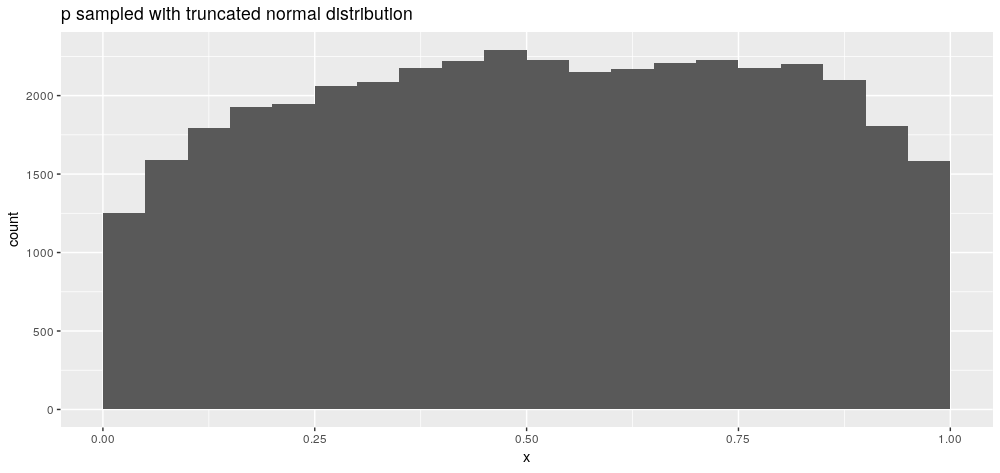
\includegraphics[width=\linewidth]{img/truncatedNormalAlsoBiased.png}
	\caption{Samples drawn using truncated normal distribution as proposal; 200 chains with 200 samples each, $\sigma = 0.1$}
	\label{fig:truncatedAlsoBiased}
\end{figure}
 
 Unfortunately, as figure \ref{fig:truncatedAlsoBiased} shows, sampling with the truncated normal distribution method also introduces bias as the samples are not uniformly distributed. 

% R code for sampling:
% x = qnorm(  pnorm(a,mu,sigma) + runif(1)*(pnorm(b,mu,sigma) - pnorm(a,mu,sigma))  

\subsubsection{Multiplicative Random Walk}
Cappé \cite{cappe} proposes an interesting class of Metropolis-Hastings-Steps which are all based on a \textit{multiplicative random walk}. Let us first consider a parameter $p$ with constraint $p \in \R_{\geq 0}$. Then let the new proposal $\tilde{p}$ be defined as 
\[
	log\left(\tilde{p}\right) := log(p) + X
\]
where $X \sim \mathcal{N}(0, \sigma)$.

\begin{lemma}
	When defined as above, we have $Q\left(log(\tilde{p}), log(p)\right) = Q\left( log(p), log(\tilde{p})\right)$.
	
	Note, that we do \textit{not} have
	\[
	Q\left(\tilde{p}, p\right) = Q\left( p , \tilde{p}\right)
	\]
\end{lemma}

	 Please note that even though $Q$ is symmetric, we need to invoke the substitution method to obtain the correct acceptance probability. 
	 In particular, note that 
	 \begin{align*}
	 	\int f(x) dx = \int_{log(exp(y))} f(x) dx &= 
	 	\int_{log(y)} \frac{1}{\sqrt{2 \pi \sigma}} e^{- \frac{ \left(exp(x) - 0\right)^2}{2 \sigma^2}} \left(exp(x)\right)^{\prime}  \, dx\\
	 	&= \int_{log(y)} \frac{1}{\sqrt{2 \pi \sigma}} e^{- \frac{ \left(exp(x) - 0\right)^2}{2 \sigma^2}} exp(x) \, dx
	 \end{align*} 
	 
	 This means that when manipulating $p$ in log-space, the acceptance ratio needs to be altered as follows\footnote{Note that this also implies that $0$ must not be part of the domain of $p$. }:
	 \[
	 	\alpha := min \Bigg\{ 
	 		1, \frac{\tip{\tilde{\Theta}}}{\tip{\Theta}} \, \frac{\tilde{p}}{p}
	 		\Bigg\}
	 \]
	 
	 \begin{figure}
	 	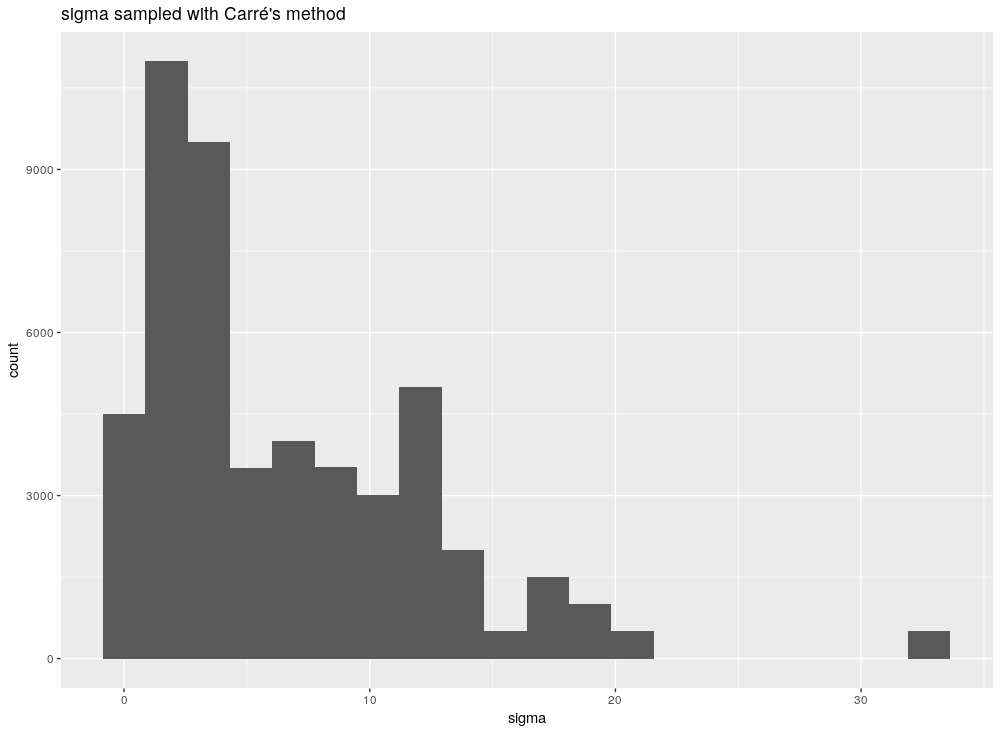
\includegraphics[height=0.3\textheight]{img/carre_sigma_biased.png}
	 	\caption{Sampling $\sigma$ by applying Metropolis-Hastings with the multiplicative random walk, 200 chains with each 200 steps and the initial sample drawn from $U[0, 10]$}
	 	\label{fig:carre_sigma_not_uniform}
	 \end{figure}
	 
	 Note that while the sampling is uniform \textit{on the log space}, it is not uniform in normal space. Figure \ref{fig:carre_sigma_not_uniform} shows a histogram of $\sigma$ sampled by the aforementioned method\footnote{the initial values are distributed as in $U[0, 10]$}. As $\sigma$ is unbounded in this case, it is indeed not possible to uniformly sample $\sigma$\footnote{There exists no unbounded, uniform distribution}. However, this methodology (needlessly) introduces a prior which is \textit{inherent} to the sampling method itself and will affect any intentional prior which might be defined in addition. 
	 
	 Cappé \cite{cappe2003} further suggests to extend this methodology to accommodate parameters $p_1, \dots, p_n \in [0,1]$ with additional constraint $\sum p_i = 1$. This is achieved by obtaining $\tilde{p_i}$ as defined above and then setting
	 \[
	 	p_i^{\prime} := \frac{\tilde{p_i}}{\sum_{j=1} \tilde{p_j}}
	 \]
	 as the new proposed value. Cappé suggests to further use $Exp(1)$-priors on $p_i^{\prime}$. 
	 
	 Note that - just as noted above, the resulting distributions are heavily \textit{biased}. Fig \ref{fig:carre_p1_p2_hist} and \ref{fig:carre_p1p2_estimated_dens} show estimated densities and histograms of $p1, p2 \in [0,1]$ with $p1 + p2 = 1$ sampled with $200$ chains each having $200$ steps and $\sigma = 0.1$, the initial values being uniformly sampled from $[0, 1]$. Please note that the sample is biased regardless of whether the proposed priors are used or not. Hence, this method of drawing numbers has an \textit{inherent prior} which will distort any extra, intended prior that could be defined in addition. 
	 
	 
 
	 \begin{minipage}{\linewidth}
	 	\centering
	 	\begin{minipage}{0.45\linewidth}
	 		\begin{figure}[H]
	 				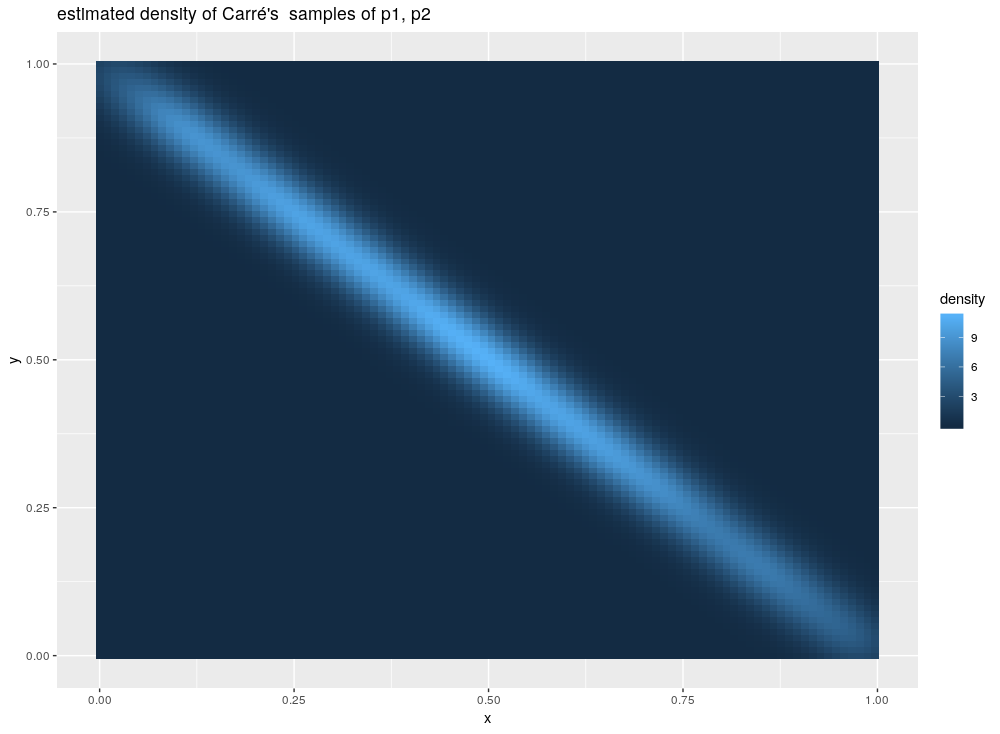
\includegraphics[width=0.9\linewidth]{img/carre_estimated_density_p1_p2.png}
	 			\caption{The estimated density of the samples p1, p2 drawn by Carré's method (200 chains, 200 steps, $\sigma = 0.1$). The samples are clearly biased towards the middle and not uniformly distributed}
	 			\label{fig:carre_p1p2_estimated_dens}
	 		\end{figure}
	 	\end{minipage}
	 	\hspace{0.05\linewidth}
	 	\begin{minipage}{0.45\linewidth}
	 		\begin{figure}[H]
	 				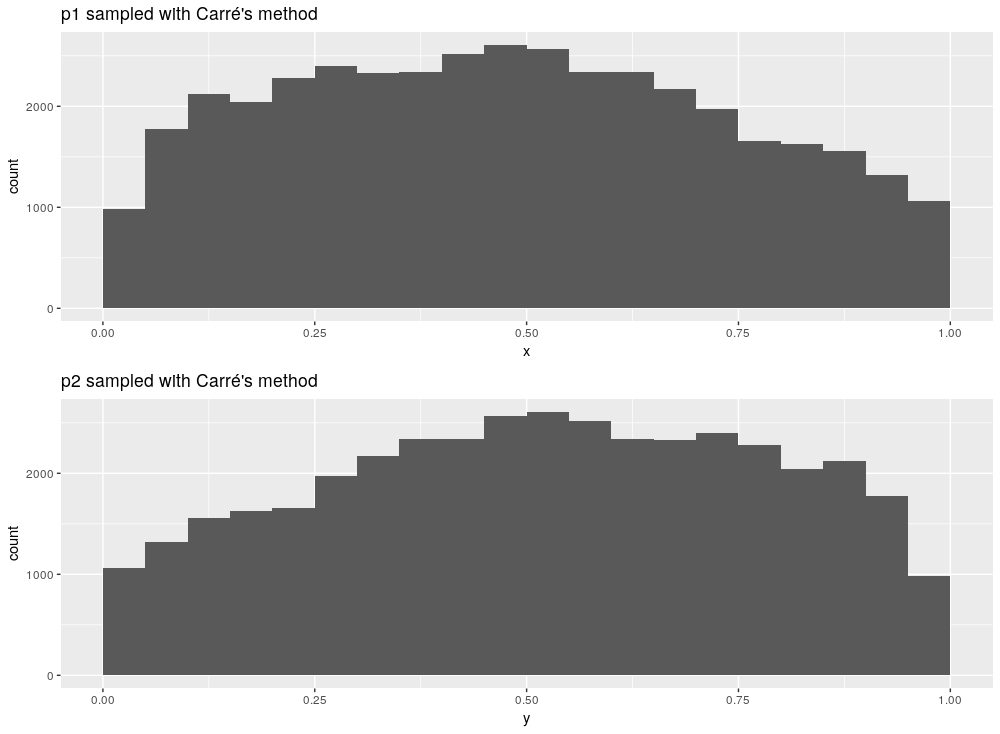
\includegraphics[width=0.9\linewidth]{img/carre_p1_p2_hists.png}
	 			\caption{The estimated histograms of the samples p1, p2 drawn by Carré's method (200 chains, 200 steps, $\sigma = 0.1$). The samples are clearly biased towards the middle and not uniformly distributed}
	 			\label{fig:carre_p1_p2_hist}
	 		\end{figure}
	 	\end{minipage}
	 \end{minipage}


 \begin{minipage}{\linewidth}
	\centering
	\begin{minipage}{0.45\linewidth}
		\begin{figure}[H]
		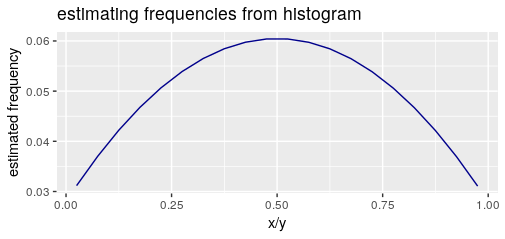
\includegraphics[width=\linewidth]{img/carreCorrectionEstimatedFrequencies.png}
		\caption{Estimated density from histogram of $x, y$ as sampled by the Carré multiplicative random walk method}
		\label{fig:estimDensity_carre_multiplicative}

		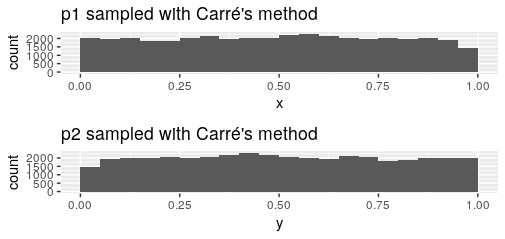
\includegraphics[width=1.0\linewidth]{img/carreCorrectedDensity.png}
		\caption{Approximately Corrected Density for Carré multiplicative random walk sampled values}
		\label{fig:carreCorrectedWorks}
		\end{figure}
	\end{minipage}
	\hspace{0.05\linewidth}
	\begin{minipage}{0.45\linewidth}
		\subsection{Corrective Measures}
		We suggest to correct for this bias by reweighting the probabilities accordingly. As the steps are normally distributed and there is no closed-form to the normal distribution, we do not expect to find an analytical solution to the sampling distribution. 
		Hence, we resort to an approximative correction. 
		
		In particular, the frequency of any given sample is estimated with the aid of the histograms shown above; the density is fitted with a polynomial of degree $2$\footnote{The actual estimated density obtained is $f(x) = 0.028 + 0.13 * x - 0.1301 * x^2$ in this case}; the result is shown in figure \ref{fig:estimDensity_carre_multiplicative}. This density is then used to correct the sampling density by a factor as follows:
	\end{minipage}
\end{minipage}

\[
\tilde{\text{samplingDensity}}(x) := \text{samplingDensity}(x) \, \frac{max_x\{ f(x) \}}{f(x)}
\]

Figure \ref{fig:carreCorrectedWorks} clearly shows that the resulting distribution is indeed much closer to the uniform distribution. 


Note that this simple, approximative method can be used for arbitrary sampling methods. While it is not necessary to correct for the ''bumping'' method, the ''bumping'' method alone can not be used to enforce contraints, for instance that the individual values some to one. 

Note also that combining the aforementioned projection method (i.e. dividing by the sum to achieve a sum to $1$) does not yield uniform results, even when applied to samples which are sampled using the ''bumping'' method. As shown above, this method generates uniformly distributed values - which are not uniform after having undergone said transformation. 

